\documentclass[border=14pt]{standalone}
\usepackage{tikz}
\usepackage{xcolor}
\usetikzlibrary{arrows.meta, positioning, fit, backgrounds}

\definecolor{cpurple}{HTML}{7F77DD}
\definecolor{cteal}{HTML}{1D9E75}
\definecolor{camber}{HTML}{BA7517}
\definecolor{cblue}{HTML}{378ADD}
\definecolor{cgray}{HTML}{5F5E5A}
\definecolor{ccoral}{HTML}{D85A30}
\definecolor{ctextd}{HTML}{2C2C2A}

\tikzset{
  box/.style 2 args={
    rounded corners=6pt,
    draw=#1!65, fill=#1!8,
    text=ctextd, font=\small\sffamily,
    minimum width=#2, minimum height=1.05cm,
    align=center, line width=0.55pt,
    inner sep=6pt,
  },
  lbl/.style={font=\footnotesize\sffamily, text=cgray},
  arr/.style={
    -{Stealth[length=5pt,width=4pt]},
    line width=0.75pt, color=cgray!70,
  },
}

\begin{document}
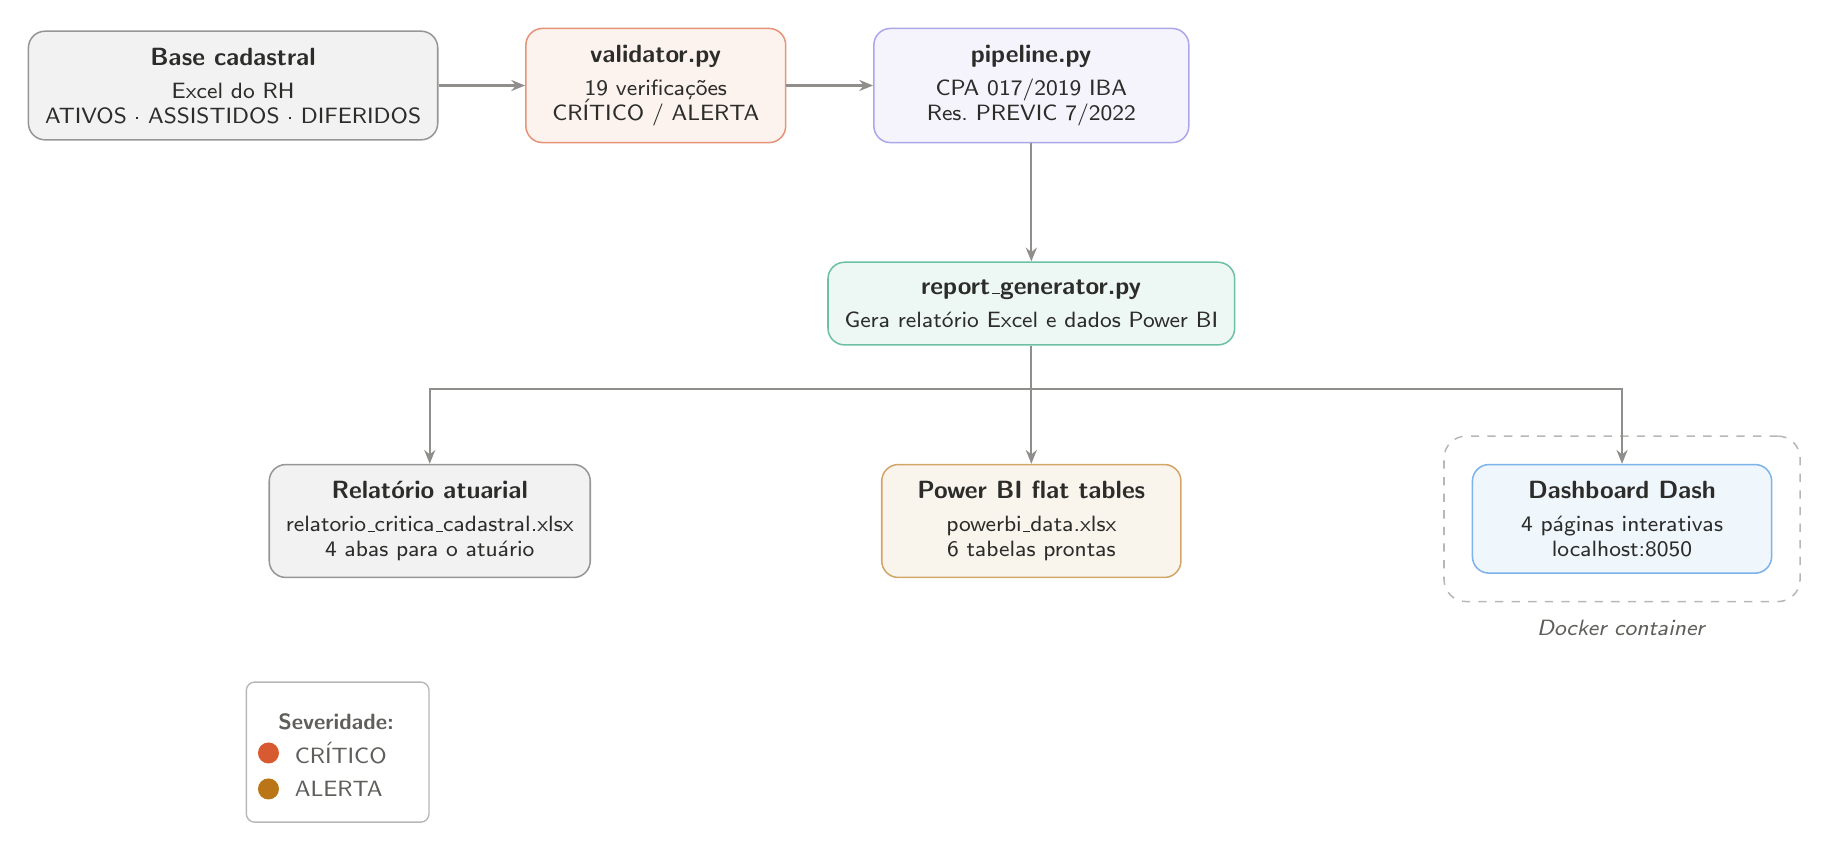
\begin{tikzpicture}[node distance=1.0cm and 1.1cm]

%% ── ROW 1 ─────────────────────────────────────────────────
\node[box={cgray}{3.5cm}] (input) {%
  \textbf{Base cadastral}\\[1pt]%
  \footnotesize Excel do RH\\[-2pt]%
  \footnotesize ATIVOS \textperiodcentered{} ASSISTIDOS \textperiodcentered{} DIFERIDOS%
};

\node[box={ccoral}{3.3cm}, right=of input] (validator) {%
  \textbf{validator.py}\\[1pt]%
  \footnotesize 19 verificações\\[-2pt]%
  \footnotesize CRÍTICO / ALERTA%
};

\node[box={cpurple}{4.0cm}, right=of validator] (pipeline) {%
  \textbf{pipeline.py}\\[1pt]%
  \footnotesize CPA 017/2019 IBA\\[-2pt]%
  \footnotesize Res.\ PREVIC 7/2022%
};

%% ── ROW 2 ─────────────────────────────────────────────────
\node[box={cteal}{4.4cm}, below=1.5cm of pipeline] (report) {%
  \textbf{report\_generator.py}\\[1pt]%
  \footnotesize Gera relatório Excel e dados Power BI%
};

%% ── ROW 3 ─────────────────────────────────────────────────
\node[box={cgray}{3.8cm}, below left=1.5cm and 3.0cm of report] (excel) {%
  \textbf{Relatório atuarial}\\[1pt]%
  \footnotesize relatorio\_critica\_cadastral.xlsx\\[-2pt]%
  \footnotesize 4 abas para o atuário%
};

\node[box={camber}{3.8cm}, below=1.5cm of report] (pbi) {%
  \textbf{Power BI flat tables}\\[1pt]%
  \footnotesize powerbi\_data.xlsx\\[-2pt]%
  \footnotesize 6 tabelas prontas%
};

\node[box={cblue}{3.8cm}, below right=1.5cm and 3.0cm of report] (dash) {%
  \textbf{Dashboard Dash}\\[1pt]%
  \footnotesize 4 páginas interativas\\[-2pt]%
  \footnotesize localhost:8050%
};

%% ── Docker dashed border ──────────────────────────────────
\node[draw=cgray!45, dashed, rounded corners=8pt, line width=0.55pt,
      fit=(dash), inner sep=10pt] (docker) {};
\node[lbl, below=3pt of docker.south] {\textit{Docker container}};

%% ── Arrows ────────────────────────────────────────────────
\draw[arr] (input)     -- (validator);
\draw[arr] (validator) -- (pipeline);
\draw[arr] (pipeline)  -- (report);
\draw[arr] (report.south) -- ++(0,-0.55) -| (excel.north);
\draw[arr] (report)       -- (pbi);
\draw[arr] (report.south) -- ++(0,-0.55) -| (dash.north);

%% ── Severity legend (anchored to excel node) ──────────────
\node[lbl, below=1.6cm of excel.south west, anchor=north west,
      xshift=0pt] (legtitle) {\textbf{Severidade:}};

\fill[ccoral]
  ([xshift=0pt, yshift=-5pt]legtitle.south west) circle (3.8pt);
\node[lbl, right=6pt of legtitle.south west, anchor=west, yshift=-5pt]
  {CRÍTICO};

\fill[camber]
  ([xshift=0pt, yshift=-18pt]legtitle.south west) circle (3.8pt);
\node[lbl, right=6pt of legtitle.south west, anchor=west, yshift=-18pt]
  {ALERTA};

\draw[cgray!45, rounded corners=3pt, line width=0.5pt]
  ([xshift=-8pt, yshift=8pt]legtitle.north west)
  rectangle
  ([xshift=58pt, yshift=-30pt]legtitle.south west);

\end{tikzpicture}
\end{document}